\subsection{Schema generale inserimento della data source}
\hspace*{-0.5cm}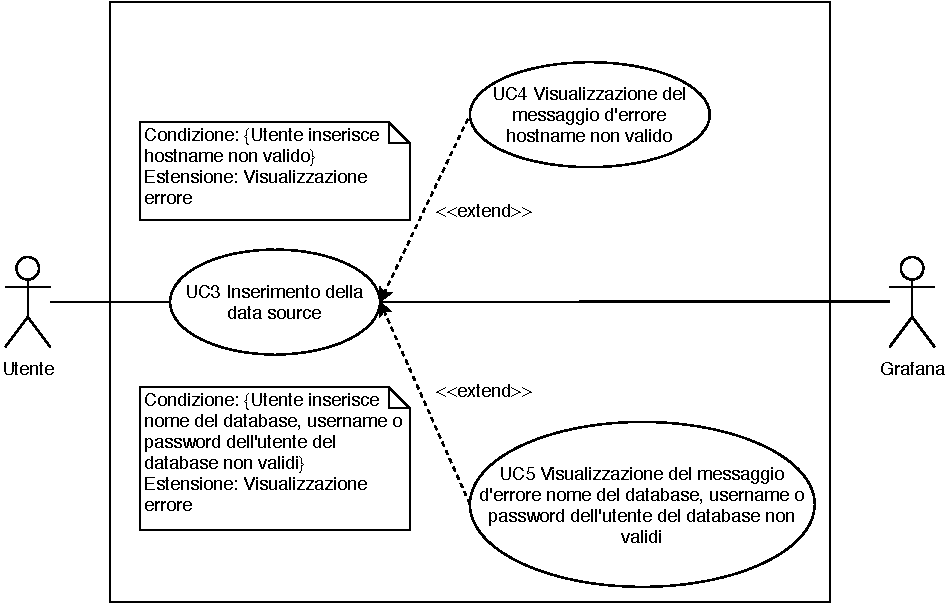
\includegraphics[width=400pt, height=300pt]{img/schema_generale_uc3.pdf}
\subsection{UC3 - Inserimento della data source}
\hspace*{-1.5cm}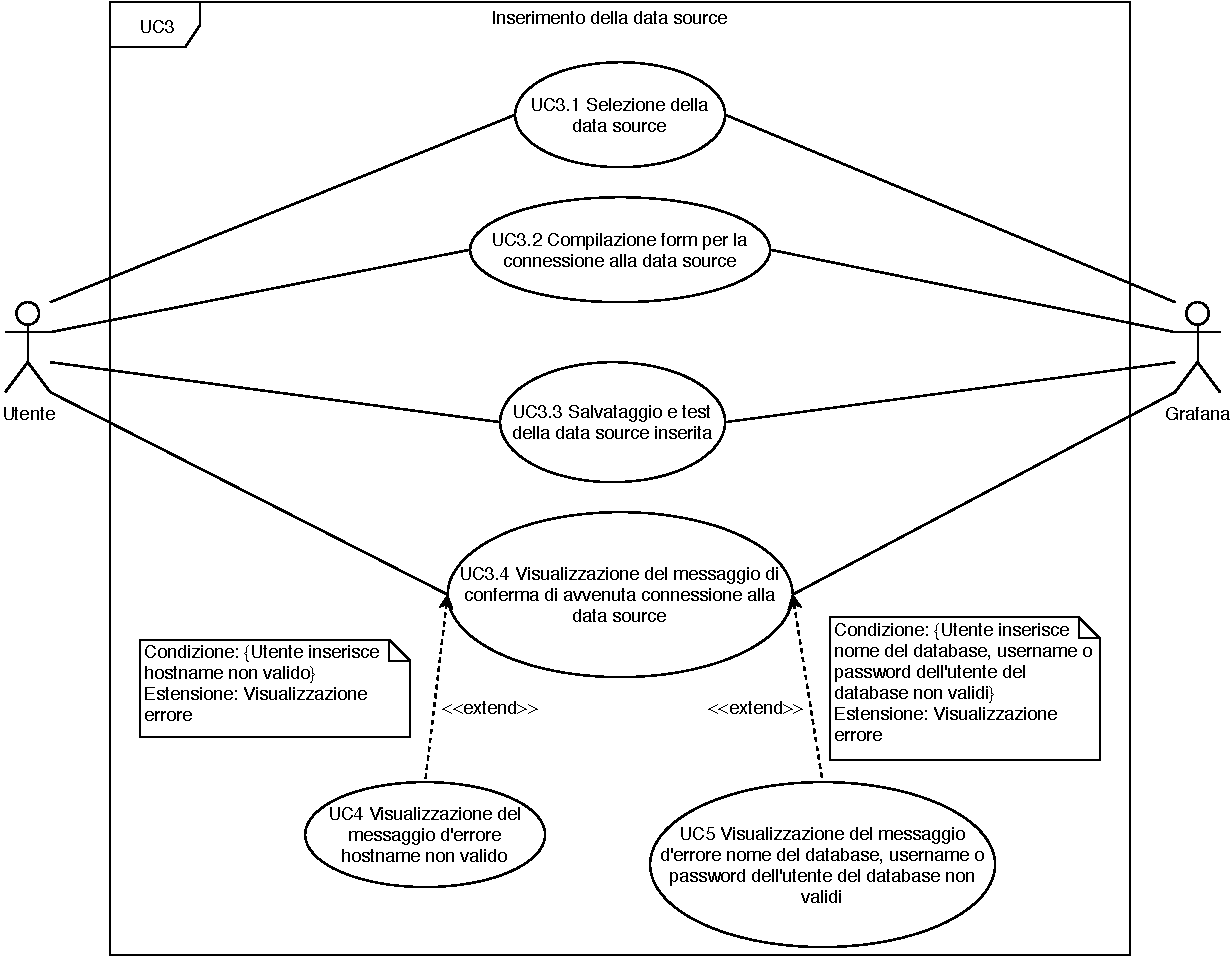
\includegraphics[width=500pt, height=400pt]{img/uc3.pdf}
\begin{itemize}
    \item \textbf{Codice identificativo}: UC3;
    \item \textbf{Titolo}: Inserimento della data source;
    \item \textbf{Attori primari}: Utente;
    \item \textbf{Attori secondari}: Grafana\glo;
    \item \textbf{Descrizione}: L'utente seleziona su Grafana\glosp una data source da dove prelevare i dati e quindi inserisce hostname, nome del database, username e                                password dell'utente del database;
    \item \textbf{Precondizioni}: L'utente deve aver effettuato il login nella piattaforma Grafana\glo;
    \item \textbf{Postcondizioni}: L'utente ha aggiunto una data source valido alla piattaforma Grafana\glo;
    \item \textbf{Scenario principale}:
    \begin{enumerate}
        \item L'utente seleziona la data source (UC3.1);
        \item L'utente inserisce i dati della data source (UC3.2);
        \item L'utente salva e testa la nuova data source (UC3.3);
        \item Visualizzazione del messaggio di avvenuta connessione alla data source (UC 3.4).
    \end{enumerate}
    \item \textbf{Estensioni}:
    \begin{enumerate}
        \item Visualizzazione del messaggio di errore hostname non valido (UC4);
        \item Visualizzazione del messaggio di errore nome del database, username o password dell'utente del database non validi (UC5).
    \end{enumerate}
\end{itemize}
    \subsubsection{UC3.1 - Selezione della data source}
        \begin{itemize}
            \item \textbf{Codice identificativo}: UC3.1;
            \item \textbf{Titolo}: Selezione della data source;
            \item \textbf{Attori primari}: Utente;
            \item \textbf{Attori secondari}: Grafana\glo;
            \item \textbf{Descrizione}: L'utente tramite le impostazioni di Grafana\glosp selezione una data source dalla lista;
            \item \textbf{Precondizioni}: L'utente deve aver effettuato il login nella piattaforma Grafana\glo;
            \item \textbf{Postcondizioni}: L'utente ha selezionato una data source;
            \item \textbf{Scenario principale}:
            \begin{enumerate}
                \item L'utente accede alla schermata delle impostazioni di Grafana\glosp dedicata alle data source;
                \item L'utente seleziona una data source dalla lista.
            \end{enumerate}
        \end{itemize}
    \subsubsection{UC3.2 - Compilazione form per la connessione alla data source}
    \hspace*{-0.5cm}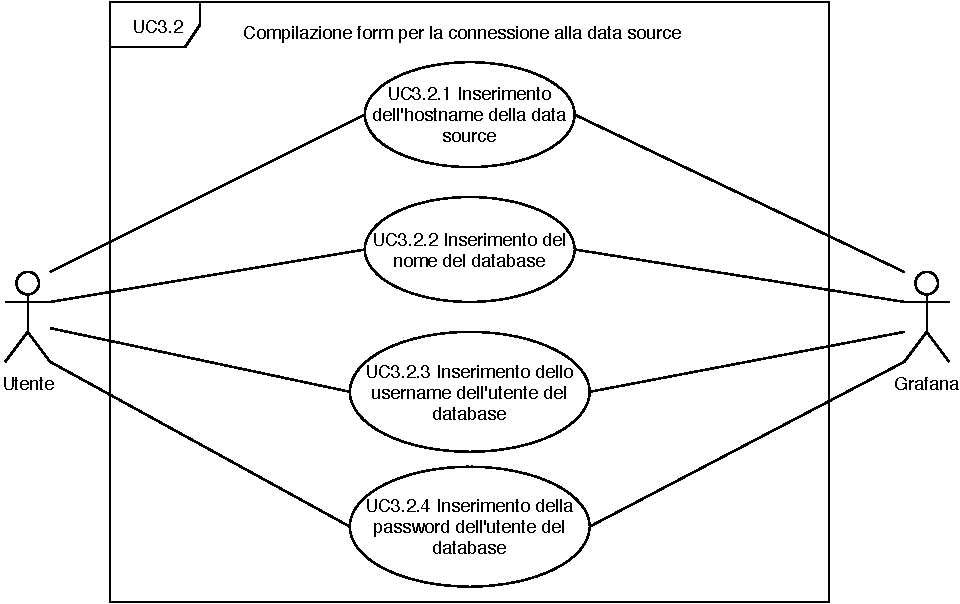
\includegraphics[width=400pt, height=300pt]{img/uc3_2.pdf}
        \begin{itemize}
            \item \textbf{Codice identificativo}: UC3.2;
            \item \textbf{Titolo}: Compilazione form per la connessione alla data source;
            \item \textbf{Attori primari}: Utente;
            \item \textbf{Attori secondari}: Grafana\glo;
            \item \textbf{Descrizione}: L'utente inserisce in un form i dati necessari alla connessione alla data source;
            \item \textbf{Precondizioni}: L'utente deve aver effettuato il login nella piattaforma Grafana\glosp e selezionato una data source valida;
            \item \textbf{Postcondizioni}: L'utente ha compilato i campi necessari alla connessione alla data source;
            \item \textbf{Scenario principale}:
            \begin{enumerate}
                \item L'utente inserisce l'hostname della data source (UC3.2.1);
                \item L'utente inserisce il nome del database (UC3.2.2);
                \item L'utente inserisce il nome utente dell'utente del database (UC3.2.3);
                \item L'utente inserisce la password dell'utente del database (UC3.2.4);
            \end{enumerate}
        \end{itemize}
        \paragraph{UC3.2.1 - Inserimento dell'hostname della data source}
            \begin{itemize}
                \item \textbf{Codice identificativo}: UC3.2.1;
                \item \textbf{Titolo}: Inserimento dell'hostname della data source;
                \item \textbf{Attori primari}: Utente;
                \item \textbf{Attori secondari}: Grafana\glo;
                \item \textbf{Descrizione}: L'utente inserisce l'hostname della data source;
                \item \textbf{Precondizioni}: L'utente deve aver effettuato il login nella piattaforma Grafana\glosp e selezionato una data source valida;
                \item \textbf{Postcondizioni}: L'utente ha inserito l'hostname della data source;
                \item \textbf{Scenario principale}: L'utente inserisce l'hostname della data source nell'apposito campo.
            \end{itemize}
        \paragraph{UC3.2.2 - Inserimento del nome del database}
            \begin{itemize}
                \item \textbf{Codice identificativo}: UC3.2.2;
                \item \textbf{Titolo}: Inserimento del nome del database;
                \item \textbf{Attori primari}: Utente;
                \item \textbf{Attori secondari}: Grafana\glo;
                \item \textbf{Descrizione}: L'utente inserisce il nome del database;
                \item \textbf{Precondizioni}: L'utente deve aver effettuato il login nella piattaforma Grafana\glosp e selezionato una data source valida;
                \item \textbf{Postcondizioni}: L'utente ha inserito il nome del database;
                \item \textbf{Scenario principale}: L'utente inserisce il nome del database nell'apposito campo.
            \end{itemize}
        \paragraph{UC3.2.3 - Inserimento dello username dell'utente del database}
            \begin{itemize}
                \item \textbf{Codice identificativo}: UC3.2.3;
                \item \textbf{Titolo}: Inserimento dello username dell'utente del database;
                \item \textbf{Attori primari}: Utente;
                \item \textbf{Attori secondari}: Grafana\glo;
                \item \textbf{Descrizione}: L'utente inserisce lo username dell'utente del database;
                \item \textbf{Precondizioni}: L'utente deve aver effettuato il login nella piattaforma Grafana\glosp e selezionato una data source valida;
                \item \textbf{Postcondizioni}: L'utente ha inserito lo username dell'utente del database;
                \item \textbf{Scenario principale}: L'utente inserisce lo username dell'utente del database nell'apposito campo.
            \end{itemize}
        \paragraph{UC3.2.4 - Inserimento della password dell'utente del database}
            \begin{itemize}
                \item \textbf{Codice identificativo}: UC3.2.4;
                \item \textbf{Titolo}: Inserimento della password dell'utente del database;
                \item \textbf{Attori primari}: Utente;
                \item \textbf{Attori secondari}: Grafana\glo;
                \item \textbf{Descrizione}: L'utente inserisce la password dell'utente del database;
                \item \textbf{Precondizioni}: L'utente deve aver effettuato il login nella piattaforma Grafana\glosp e selezionato una data source valida;
                \item \textbf{Postcondizioni}: L'utente ha inserito la password dell'utente del database;
                \item \textbf{Scenario principale}: L'utente inserisce la password dell'utente del database nell'apposito campo.
            \end{itemize}
    \subsubsection{UC3.3 - Salvataggio e test della data source inserita}
        \begin{itemize}
            \item \textbf{Codice identificativo}: UC3.3;
            \item \textbf{Titolo}: Salvataggio e test della data source inserita;
            \item \textbf{Attori primari}: Utente;
            \item \textbf{Attori secondari}: Grafana\glo;
            \item \textbf{Descrizione}: L'utente salva e testa la data source inserita;
            \item \textbf{Precondizioni}: L'utente deve aver effettuato il login nella piattaforma Grafana\glo, selezionato una data source valida e inserito tutti i                                   campi sopracitati;
            \item \textbf{Postcondizioni}: L'utente ha salvato e testato una nuova data source;
            \item \textbf{Scenario principale}: L'utente salva la nuova data source che viene automaticamente testata da Grafana\glosp per verificarne il funzionamento.
        \end{itemize}
    \subsubsection{UC3.4 - Visualizzione messaggio di conferma di avvenuta connessione alla data source}
        \begin{itemize}
            \item \textbf{Codice identificativo}: UC3.4;
            \item \textbf{Titolo}: Visualizzione messaggio di conferma di avvenuta connessione alla data source;
            \item \textbf{Attori primari}: Utente;
            \item \textbf{Attori secondari}: Grafana\glo;
            \item \textbf{Descrizione}: L'utente visualizza il messaggio di conferma di avvenuta connessione alla data source;
            \item \textbf{Precondizioni}: L'utente deve aver effettuato il login nella piattaforma Grafana\glo, selezionato una data source valida e inserito tutti i                                   campi sopracitati;
            \item \textbf{Postcondizioni}: L'utente ha inserito correttamente una nuova data source a Grafana\glosp ed è connesso ad essa;
            \item \textbf{Scenario principale}: L'utente visualizza il messaggio di conferma di avvenuta connessione alla data source.
        \end{itemize}
\subsection{UC4 - Visualizzazione del messaggio di errore hostname non valido}
\begin{itemize}
    \item \textbf{Codice identificativo}: UC4;
    \item \textbf{Titolo}: Visualizzazione del messaggio di errore hostname non valido;
    \item \textbf{Attori primari}: Utente;
    \item \textbf{Attori secondari}: Grafana\glo;
    \item \textbf{Descrizione}: L'utente visualizza il messaggio di errore che lo avvisa di aver inserito un hostname non valido;
    \item \textbf{Precondizioni}: L'utente deve aver effettuato il login nella piattaforma Grafana\glo, selezionato una data source valida e inserito almeno l'hostname;
    \item \textbf{Postcondizioni}: L'utente visualizza il messaggio di errore che lo avvisa di aver inserito un hostname non valido, annullando pertanto la connessione                                  alla data source;
    \item \textbf{Scenario principale}: L'utente visualizza il messaggio di errore che lo avvisa di aver inserito un hostname non valido.
\end{itemize}
\subsection{UC5 - Visualizzazione del messaggio di errore nome del database, username o password dell'utente del database non validi}
\begin{itemize}
    \item \textbf{Codice identificativo}: UC5;
    \item \textbf{Titolo}: Visualizzazione del messaggio di errore nome del database, username o password dell'utente del database non validi;
    \item \textbf{Attori primari}: Utente;
    \item \textbf{Attori secondari}: Grafana\glo;
    \item \textbf{Descrizione}: L'utente visualizza il messaggio di errore che lo avvisa di aver inserito un nome del database, username o password dell'utente                                       del database non validi;
    \item \textbf{Precondizioni}: L'utente deve aver effettuato il login nella piattaforma Grafana\glo, selezionato una data source valida e inserito almeno l'hostname                                 corretto, sbagliando invece la compilazione di almeno uno degli altri campi;
    \item \textbf{Postcondizioni}: L'utente visualizza il messaggio di errore che lo avvisa di aver inserito un nome del database, username o password dell'utente del                                   database non validi, annullando pertanto la connessione alla data source;
    \item \textbf{Scenario principale}: L'utente visualizza il messaggio di errore che lo avvisa di aver inserito un nome del database, username o password dell'utente                                       del database non validi.
\end{itemize}